% ----------------------------------------
% Geolocation for the Internet of Things using LoRaWAN
% Third Year Project
% Daniel Saul - 2017
% daniel.saul.14@ucl.ac.uk
% ----------------------------------------
% Set up the document class for an article
\documentclass[a4paper]{report}
\usepackage[left=1.0in, right=1.0in, top=1.5in, bottom=1.5in]{geometry}

\setlength{\parskip}{1em}

%\usepackage{savetrees}

% This packages permits using $ \therefore $
\usepackage{amssymb}
\usepackage{graphicx}

% This package allows the use of $ \text{} $
\usepackage{amsmath}

% The document title and author
\title{Multilateration based system for localization of nodes with LoRaWAN}
\author{Daniel Saul\\University College London\\ \\Supervisor: Dr Miguel Rio}

% Document header
\usepackage{fancyhdr}
\pagestyle{fancy}
\fancyhead[R]{}
\renewcommand{\chaptermark}[1]{%
    \markboth{\MakeUppercase{%
    \chaptername\ \thechapter.%
    \ #1}}{}}
\fancyhead[L]{\leftmark}
\renewcommand{\headrulewidth}{0pt}


% Begin the document
\begin{document}
    \maketitle

% Insert the abstract for the document here
\pagestyle{fancy}

\begin{abstract}
    I wish I were an abstract.
\end{abstract}

\tableofcontents


\chapter{Introduction}

  The Internet of Things (IoT) is one of the most hyped of technology buzzwords at the moment but the term was coined as long ago as 1999 by Kevin Ashton. Back then, all data on the internet was generated or uploaded by humans, whether text, images or information. But Ashton envisioned a future of computer systems generating and collating data on their own, with little to no input from us. Today we are in the situation where

  \section{Low Power Wide Area Networks}

  \section{LoRaWAN}
    \subsection{Things Connected}

  \section{Motivations}

  \section{Project Outline}

\chapter{Localization}

  \section{Received Signal Strength}

  \section{Angle of Arrival}

  \section{Time of Arrival}

  \section{Time Difference of Arrival}
    \subsection{TDOA Equations}
    \subsection{Hyperbolic Solver Algorithms}
    \subsection{Problems}

\chapter{Implementation}

  This chapter will describe the implemented test setup, ranging from the hardware through to the software and data gathering. The setup consists of a simple custom node, the existing Things Connected LoRaWAN infrastructure across London and custom server-side software. The node transmits its real location as calculated by the on-board GPS which is received by LoRaWAN gateways and uploaded to the server. These real coordinates of the transmission location can then be later compared to the estimated location by the multilateration algorithm.


  \section{Node Hardware}

    \begin{figure}
    \centering
    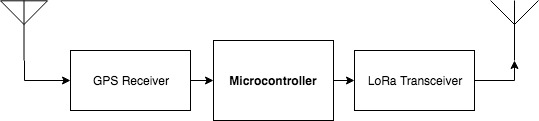
\includegraphics[width=12cm]{figures/node.jpeg}
    \caption{Node Diagram}
    \label{fig:node}
    \end{figure}

    A simple node was designed, built and programmed in C, consisting of an ESP8266 microcontroller, u-blox MAX8C GPS receiver and a Microchip RN2483 LoRa transceiver, as shown in figure \ref{fig:node}. The RN2483 was chosen as it implements the full LoRaWAN stack on-board, reducing the complexity of the microcontroller code. The GPS receiver used a basic chip antenna whilst the LoRA transceiver used an 868MHz 'rubber ducky' antenna. The specific hardware is not particularly important however, but rather the functionality is.

    The GPS receiver was configured to pedestrian mode since the primary method of testing would be a person walking with the node, as opposed to a flight or high velocity mode. The LoRaWAN configuration parameters (device address, network session key and application session key) were hard-coded into the microcontroller firmware.

    The microcontroller follows a basic loop. In each iteration, set at roughly every 10 seconds, the microcontroller requests data from the GPS (latitude, longitude, altitude, number of satellites and time) and loads it into a struct datatype. A counter in the microcontroller's flash memory, such that it is persistent across power cycling, is incremented and also added to the struct. The entire 20 byte struct is then transmitted as a binary blob payload by the LoRa transceiver. Other functionality allowing transmission on a button press and short bursts of continuous data transmission was also implemented but not ultimately used.

    The main file of the node firmware can be seen in appendix \ref{ap:nodefirmware}.


  \section{Server-side Software}

    \begin{figure}
    \centering
    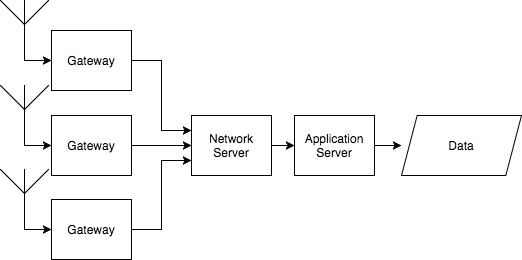
\includegraphics[width=12cm]{figures/server.jpeg}
    \caption{LoRaWAN to Server Diagram}
    \label{fig:server}
    \end{figure}

    When a gateway receives a packet from a node, it uploads it to the network server. The data can then be passed by the network server over an HTTP connection to the relevant application server, if the application server has implemented the necessary JSON-RPC methods \cite{EverynetAPI}. A python script to be run on a public server with open port 8080 is found in appendix \ref{ap:servereverynet} and implements the 'uplink' and 'post\_uplink' methods. The 'uplink' method provides data as soon as one gateway has received a packet whilst the 'post\_uplink' method should provide data on all receiving gateways a few seconds later. Unfortunately after testing, it was found that this latter method is not functional and that therefore obtaining details on all gateways is not possible this way. Hopefully it will be in the future.

    Therefore, a workaround was found by using the unofficial API running the Things Connected dashboard. The last 20 received packets from each gateway are available from a 'messages' endpoint. By continuously polling this endpoint at a rate faster than that at which the node is transmitting, all data from all gateways can be collected. Figure \ref{fig:server} shows a simplified system diagram for the LoRaWAN and server-side systems. A python script to perform an HTTP POST request to login and continually fetch data from the unofficial API through HTTP GET requests is found in appendix \ref{ap:serverfetch}. The fetched data is published to a Redis Pub/Sub channel which is subscribed to by another script, found in appendix \ref{ap:serverprocess}, where the data is processed. The payload of each packet is decoded and the binary blob unpacked into the constituent pieces of data. If the packet payload already exists in the Redis database, the details of the new gateway receiving the packet is appended to the gateway list. If it doesn't already exist, the entire packet data is freshly inserted into the database.

    It is at this point in the system that any final positioning algorithm would ultimately be included. Instead, another python script, in appendix \ref{ap:serverexport}, allows all the received data to be exported from the database to a JSON file for analysis and testing.



\chapter{Data Analysis \& Results}

  In this chapter, the gathered data and the various transformations, algorithms and analytics carried out will be presented alongside the final positioning errors obtained.

  \section{Gathered Data}

    The GPS node was taken for a walk through central London, through both areas with a high number and low number of gateways. Table \ref{tab:gatewaynums} shows the number of gateways that each packet was received by, with 648 packets received in total by 8 different unique gateways. It can be seen that only about 25\% of packets were received by 3 or more gateways, with three gateways being the minimum requirement to estimate a 2-dimensional position.

    Figure \ref{fig:datamap} provides a geographical visualization of the data. The location of each gateway that received a packet is shown in blue, the true location of packets received by less than 3 gateways are shown in red and the true location of packets received by 3 or more gateways are shown in green. With a cursory glance, it can be seen that generally more packets are received by higher numbers of gateways in areas of high gateway density.

    \begin{table}[h]
      \begin{center}
        \caption{Number of packets received by n gateways}
        \begin{tabular}{|c|c|c|c|c|c|c|}
          \hline
          Number of Gateways & 1 & 2 & 3 & 4 & 5 & Total \\
          \hline
          Number of Packets & 310 & 168 & 111 & 46 & 13 & 648 \\
          \hline
        \end{tabular}
      \end{center}
      \label{tab:gatewaynums}
    \end{table}

    \begin{figure}[h]
    \centering
    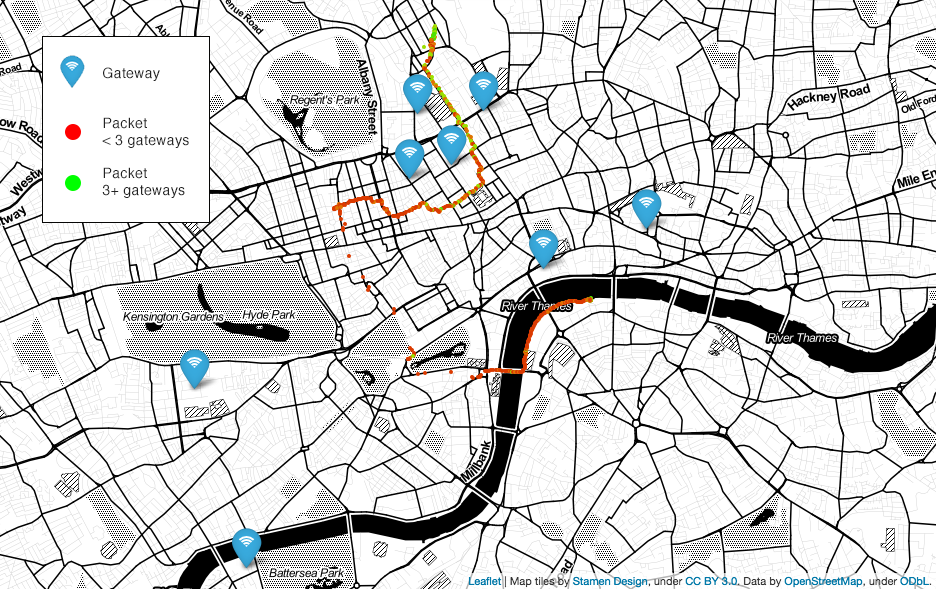
\includegraphics[width=12cm]{figures/map_data.png}
    \caption{Geographical visualization of gathered data}
    \label{fig:datamap}
    \end{figure}


  \section{Cartesian Coordinates}
    When working with the TDOA algorithms, it is important that a linear cartesian coordinate system is used, as opposed to the WGS84 latitude and longitude used by the GPS.

    If 3-dimensional positioning was required, latitude, longitude and altitude (LLA) could be converted to the Earth Centred, Earth Fixed (ECEF) frame and vice versa. In this reference frame, the origin is at the centre of the Earth with the x-axis intersecting the Greenwich meridian and the equator, the z-axis being along the spin axis of the Earth and the y-axis being perpendicular to both of these. However, for 3-dimensional position estimates, a minimum of 4 gateways would be required and the effect of altitude is likely to be negligible compared to other sources of error.

    For 2-dimensional positioning, a local grid reference frame can be used. Latitude and longitude can be converted to OSGB36, the British Ordnance Survey National Grid reference system, and vice versa, through a number of calculations and adjustments detailed in OSTN02 \cite{OSTN02}. The resulting cartesian coordinates are in metres and also allow for easy plotting of the hyperbolic equations and position estimates. When positioning errors and distances are given, it is simply the euclidean distance between two sets of (x,y) coordinates in metres.





\chapter{Conclusion}

  Since only 50\% of packets were received by 3 or more gateways and a further x\% were rejected, leaving only y\% of packets with location estimates, it is clear that the LoRaWAN network used is not ideal for positioning. However, it is important to note this is a relatively new network and that with a broader spread of gateways, these numbers are likely to be greatly improved. It should also be noted that investigating the number of receiving gateways and distance from gateways was not a primary aim and ideally more data representing a greater geographical spread around the network's gateways would be collected.




% Example Chapter for Stuff
\chapter{Example Chapter}

  \section{Aims}
  I aim to do things, as shown in equation (\ref{eq:myeq}). I will show how to do this in Section \ref{app}.

  \begin{equation}
  \label{eq:myeq}
  f(x) = \dot{x} + B u(t) + C x(x)
  \end{equation}


  \section{Apparatus}
  \label{app}

  	50\% of my study.

      A diagram of how to set up the apparatus is shown in figure \ref{fig:app}.

      \begin{figure}
      \centering
      %\includegraphics[height=5cm]{blank}
      \caption{Apparatus setup}
      \label{fig:app}
      \end{figure}

  \section{Observations}

  %This was demonstrated in \cite{Bonfils2014}.

  \section{Discussion}

      These results can be seen in table \ref{fig:myt}.

      \begin{table}
      \begin{center}
      \caption{Predicted and measured beam deflections}
      \begin{tabular}{|c|c|c|c|}
  	\hline
  	Thing & thing & thing & thing \\
  	\hline
  	Another & another & another & another \\
  	\hline
      \end{tabular}
      \end{center}
      \label{fig:myt}
      \end{table}


% Bibliography
\bibliographystyle{unsrt}
\bibliography{references}

% Appendix
\appendix
\chapter{Node Firmware} \label{ap:nodefirmware}

\chapter{Server-Side Software}
  \section{Python Everynet API Script} \label{ap:servereverynet}
  \section{Python Fetch Script} \label{ap:serverfetch}
  \section{Python Processing Script} \label{ap:serverprocess}
  \section{Python Export Script} \label{ap:serverexport}

\end{document}
